\unnumberedchapter{Introduction}

The ability of reasoning in a tridimensional space if of paramount importance for any agent in our physical world.
Very early in the evolutionary process, living beings developed mechanisms for sensing the world
in 3D.
Birds, mammals, reptiles and even insects: they all developed some type of \emph{stereopsis} --
the ability to perceive 3D from multiple views.
Since evolution showed us that living beings benefit from 3D reasoning, it makes sense that man-made
agents should be endowed with similar capabilities.
If we want to build machines that can interact with the world around us, grasp objects, avoid obstacles and reason about the space in general, we need to be able build models that allow those machines
to analyze and generate 3D data.
This thesis is focused on developing techniques that allow us to build those models in a variety of scenarios, with a specific focus on deep learning techniques.

We are mainly concerned about two important issues: \emph{representation} and \emph{data}.
Regarding representations, differently from images, it is not clear what is the best way
to represent 3D data in deep learning models.
The first part of this thesis (Chapters 1, 2 and 3) focuses on unstructured representations.
We show how we can build models capable of generating 3D data represented as sets of point clouds
(Chapters 1 and 2) and shape handles (Chapter 3).
Point cloud models have a smaller memory footprint than volumetric and multiview counterparts while
reconstructing more accurate shapes; models based on sets of shape handles have a different goal -- they are designed be
amenable to shape manipulation tasks, like editing and completion.
The second part of this thesis concerns dealing with the lack of 3D data as supervision and
understanding what is the role that neural network architectures play in inducing shape priors.
Chapter 4 describes how to utilize approximate convex decomposition (ACD) as self-supervised learning task
to improve discriminative models of point clouds trained with limited amount of labels.
We show that features learned by computing ACD yield significant improvement in few-shot segmentation
and unsupervised shape classification benchmarks.
Chapters 5 and 6 explore the prior induced by neural networks when generating 3D data.
Chapter 5 studies the case where networks are used to represent manifolds.
We analytically characterize this prior by analyzing the networks' limiting behavior as a Gaussian
Process and show that it yields impressive results in surface reconstruction tasks.
On the other hand, Chapter 6 is focused on reconstructing shapes using volumetric representations
while learning directly from images.
We introduce a series of differentiable projection operators and show applications to
shape reconstruction from silhouettes, depth images and computational tomography.
Chapter 7 builds upon some these operators to tackle a more challenging problems:
lear generative models of 3D data when no 3D or viewpoint information is available.
More preciselly, we present a class of generative adversarial networks, named \prgans, that is
capable of generating 3D shapes from a collection of \emph{unlabeled} images.
Finally, Chapter 8 presents a proposal to leverage some of the techniques developed during
this thesis in more realistic applications.
Instead of using object-oriented approaches as done in the rest of thesis, we plan to investigate
models to generate scenes from single RGB images.
More importantly, we want to train these models using multiple modalities of supervision:
from full 3D information to image level annotations like semantic masks or keypoints.
The next sections will dive into the two main parts of this thesis in more detail.


\section*{Learning from Unstructured Data}

Tridimensional occupancy grids are a natural choice for representing 3D data in deep neural networks.
They are a straightforward extension to raster images and convolutional layers can be seamlessly
applied to this type of data.
Another way to represent 3D data is by simply utilizing multiple 2D images of a 3D object.
We refer to this as multi-view representation.
This type of representation can also be easily integrated with convolutional layers and even
offers the extra advantage of being able to leverage image features pre-trained from massive image
datasets.

\begin{figure}
 \begin{center}
 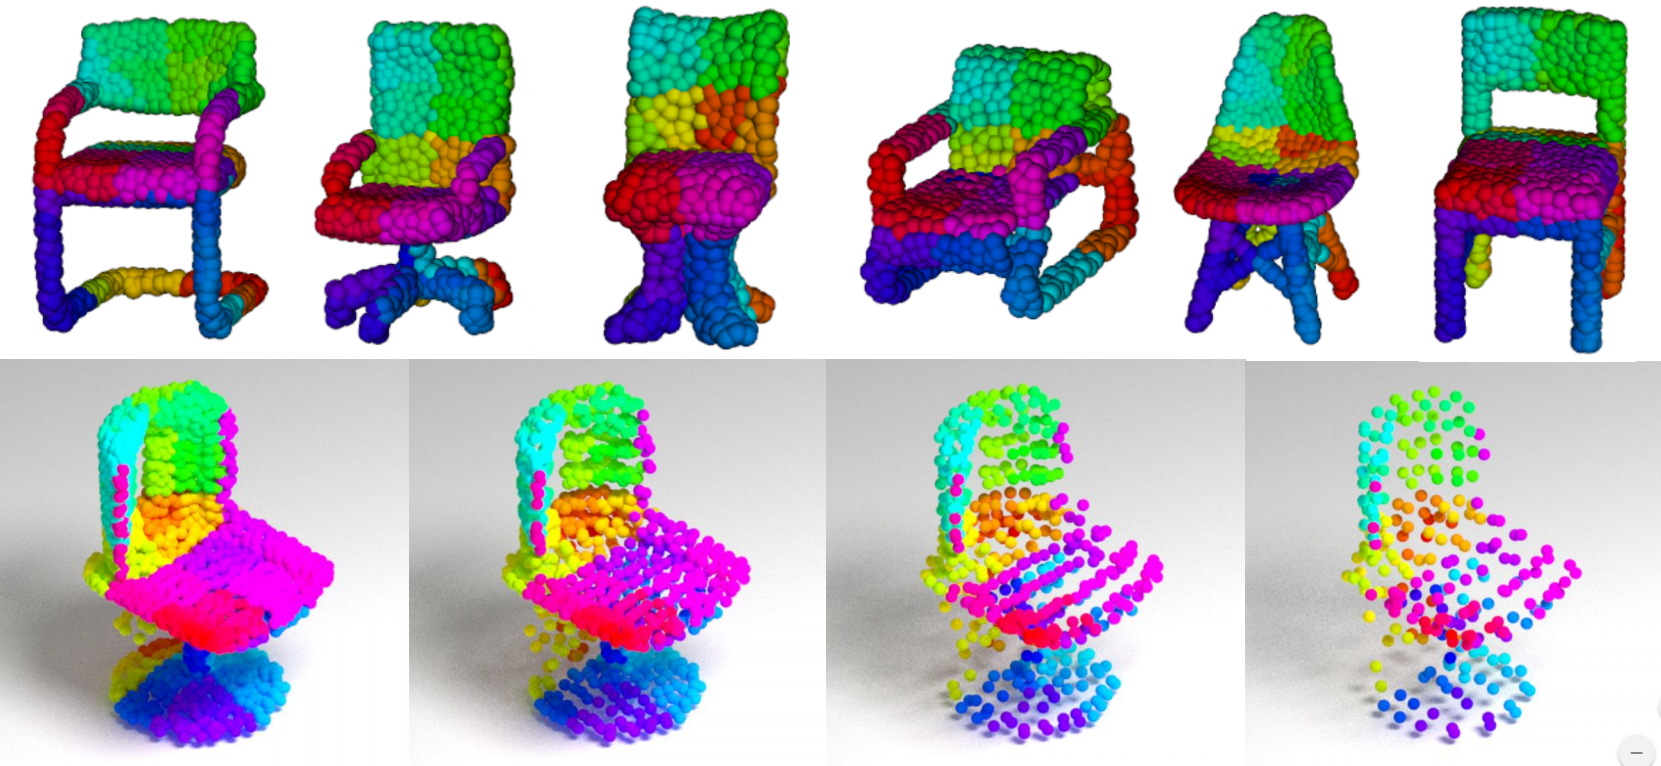
\includegraphics[width=0.7\linewidth]{figs/shapepartition.png}
 \end{center}
 \vspace{-20pt}
 \caption{\small Point clouds sorted according to spatial partitioning structures induce
 reasonable point correspondence (indicated by similar colors).
 The same structure can also be used to compute multiple point cloud resolutions.
 We build upon these observations to design multi-resolution convolutional operators
 for point cloud data.}
\end{figure}

However, generating 3D shapes poses a more challenging situation.
While generating 3D data, we are primarily concerned about generating surfaces, which are
inherently sparse in the 3D space.
This leads to a big drawback for occupancy grids: models using them require huge amounts of memory,
being prohibitively large when generating high-resolution shapes.
For multi-view representations, there are two main issues:
first, these representations are restricted to representing only the visible portion of the surface --
interior parts are not represented.
Second, it is not clear how to enforce consistency between different views, which leads to a reduced quality in the generated shapes.
Nevertheless, these models are still very memory intensive and do not handle generating
multiple categories of objects.

A reasonable alternative to those 3D representations is utilizing point clouds.
Point clouds are a very compact surface representation -- every point in the point must be part of the surface.
They also naturally support extra surface attributes, like color and normals, and are directly captured by a variety of 3D sensors.
The biggest challenge while using point clouds in deep networks lies in its unstructured nature.
Since they are sets of points, point cloud representations need to be invariant to permutations.
Moreover, differently form multi-view representations and occupancy grids, it is not clear what is the best way to use convolutional layers in point cloud data.

Our attempt in creating generative models for point clouds was bootstrapped by using spatial-partitioning data-structures to assign an approximate correspondence between points of
different point clouds~\cite{pcagan}.
The motivation is simple: if one can induce such correspondence, point clouds can be treated as structured data.
In practical terms, we compute a $kd$-tree for every point cloud and sort the points according to a level-order traversal in the leaves of the tree.
This sorting induces a reasonable correspondence between points, as shown in Figure 1.
Using this correspondence, we compute a linear low-dimensional shape representation that were used to
train the first Generative Adversarial Networks (GANs) for point cloud generation~\cite{pcagan} (\textbf{Chapter 1}).
Later, we noticed that the spatial partitioning induces a local neighborhood that can be successfully
used to define convolutional operations and to represent multiple point cloud resolutions~\cite{mrt} (\textbf{Chapter 2}).
\begin{figure}
\vspace{-20pt}
 \begin{center}
 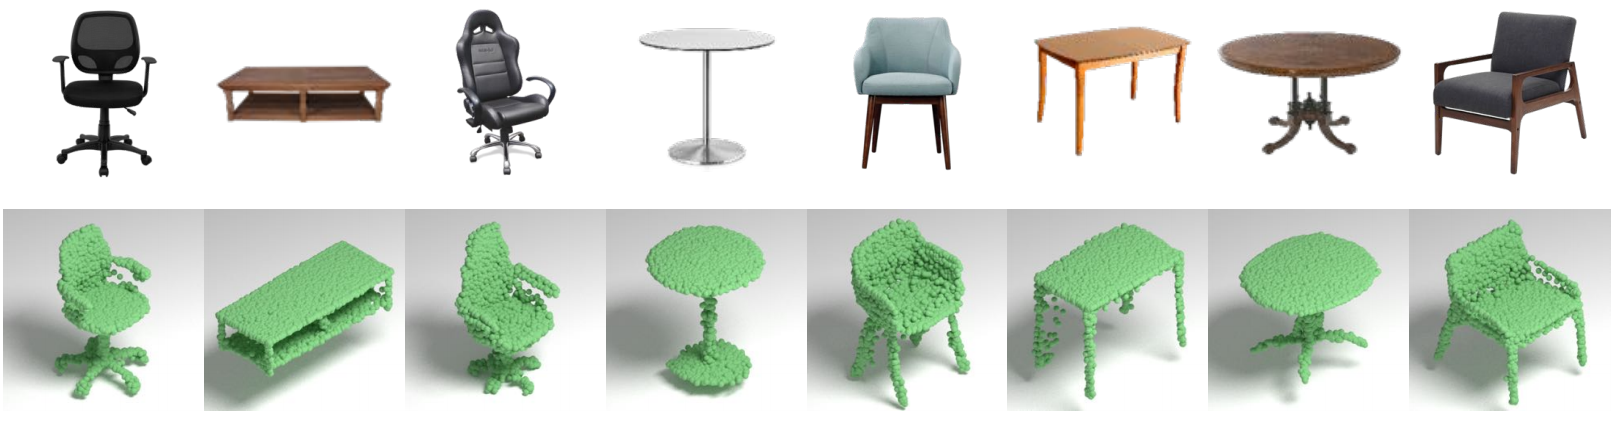
\includegraphics[width=0.7\linewidth]{figs/mrtresults.png}
 \end{center}
 \vspace{-20pt}
 \caption{\small Single-view reconstruction using MRTNets.}
 \vspace{-5pt}
\end{figure}
We called these models Multi-Resolution Tree Networks (MRTNets) and applied them to a variety of
discriminative and generative tasks, like shape classification, 
part segmentation, single-view reconstruction and VAEs.
Some of the results are presented in Figure 2.
The models have a small memory footprint when compared against multi-view and occupancy grids counterparts while yielding state-of-the-art results for point cloud classification, single-view reconstruction and
unsupervised feature learning benchmarks.

However manipulating shapes represented as point clouds is a complicated task.
Suppose one wants to edit the wings of an airplane and make them a bit larger.
If the airplane is represented as a set of points that means manually selecting and displacing
a big number of elements, which is a very laborious, borderline unfeasible task.
To this end, multiple techniques have been developed to summarize 3D shapes a set of
simpler shapes that are amenable to manipulations.
We refer to those as \emph{shape handles}.
Thus, we build upon our previous point cloud work and develop generative models capable
of creating shapes represented as sets of shape handles~\cite{shapehandles} (\textbf{Chapter 3}).
We show how those models can be trained an utilized in applications like
shape editing, creation, parsing and interpolation.


\section*{Learning with Limited 3D Supervision and Shape Priors}

Gathering 3D data is a laborious task.
Popular 3D shape benchmarks are orders of magnitude smaller than their image counterparts.
In this context, building models and training strategies that rely in less training data is specially
important.
In this thesis, we tackle this problem in multiple manners.

We start by investigating discriminative models for 3D data trained with limited amount of labels.
Simply gathering 3D data is by itself a problem, but labeling such data is equally problematic.
While many methods have been developed to improve the efficiency of labeling tasks for 3D shapes,
it is still highly desirable to develop label-efficient models that can leverage data from vast
unlabelled shape repositories.
To this end, we propose to utilize Approximate Convex Decomposition (ACD) as a self-supervised task for
training neural networks (\textbf{Chapter 4}).
We show how point cloud architectures can learn ACD by posing it as a metric learning problem trained using automatically computed labels from raw shape representations (meshes, volumes or point clouds). 
Our experiments indicate that multiple neural networks architectures trained in this fashion achieve
state of the art results in few shot part segmentation and unsupervised shape classification benchmarks.

Another way to tackle the lack of 3D data available is to investigate the role of neural
network architectures as priors for shape generation.
For images, recent work~\cite{dip} has showed that convolutional architectures induce natural image priors
that allow them to be used for multiple reconstruction tasks without requiring any training data.
We investigate an analogous behavior for two types of 3D representations in different contexts.
We start by describing how some popular neural network architectures for shape generation can be
posed as manifold parametrizations and induce useful priors for manifold reconstruction
(\textbf{Chapter 5}).
We further analyze the limiting behavior of those models as Gaussian Processes (GPs) and
analytically characterize such prior by deriving its kernel.
We also develop regularization techniques that further improve shape reconstructions in setups
with and without training data.
In the following chapter, we use convolutional architectures to generate volumetric shape
representations coupled with differentiable projection operators to reconstruct shapes from
a set of images~\cite{deepshapeprior} (\textbf{Chapter 6}).
We show how volumetric priors induced by those convolutional architectures can be used in applications
like shape reconstruction from silhouettes, depth maps, and computational tomography.

Finally, we investigate how to utilize image supervision to train 3D generative models.
As mentioned before, image data is considerably more prevalent than 3D.
For example, the most used shape classification benchmark, ModelNet40, contains about 10 thousand shapes,
whereas the most popular image classification benchmark, ImageNet, contains about 14 million images.
Nevertheless, images usually contain real world entities which are inherently 3D.
In other words, a lot of 3D information is encoded in images and being able to leverage that information
to learn to generate 3D shapes is key to build models that can overcome the lack of 3D training data.
We study this issue within a very challenging problem setup.
Consider a set of silhouette images like the ones in Figure 3.
Those images represent silhouettes of various objects from the same category.
If we have viewpoint annotation and object identification (i.e. which images correspond to the same object) this problem can be easily solved using visual hull, which corresponds to the setup
analyzed in Chapter 6.
We can make the problem harder by assuming that no viewpoint annotation is available.
In that case, we can probably achieve a reasonable result by relying in Structure from Motion (SfM) techniques.
The most difficult setup occurs when we neither have object identification nor viewpoint annotation.
In this scenario, one can only rely on non-rigid SfM, which require a strong prior over the generated shapes.
What happens when we have no information regarding 3D shapes? Can we still do something about it?


\begin{figure}
\vspace{-20pt}
 \begin{center}
 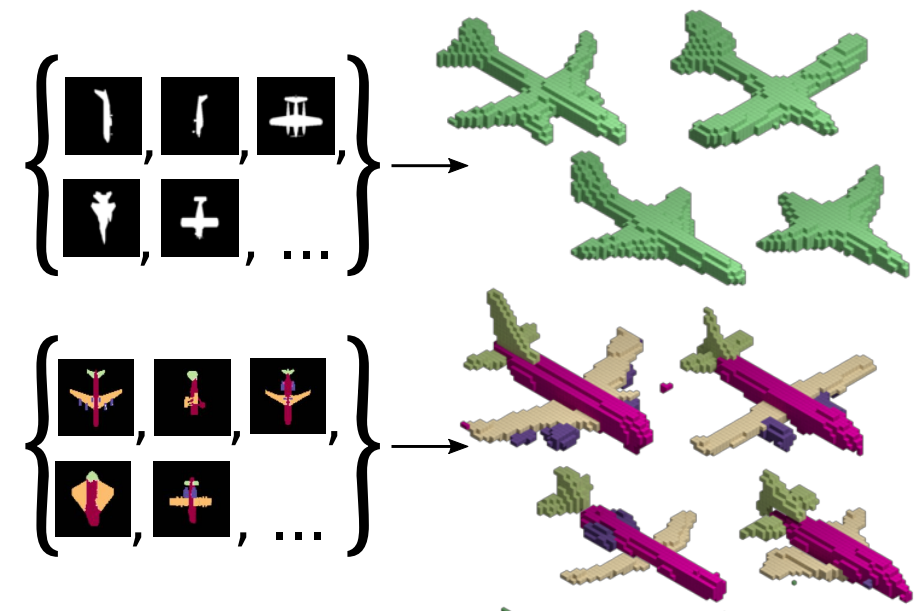
\includegraphics[width=0.8\linewidth]{figs/prganpp.png}
 \end{center}
 \vspace{-20pt}
 \caption{\small \prgan is capable of learning generative models of 3D data without using any 3D supervision.
 The core of the approach is the utilization of differentiable projection operators
 that turn 3D representation into images of silhouettes and segmentation masks.}
 \vspace{-5pt}
\end{figure}
Our solution consists of utilizing deep generative models coupled with some of the differentiable projection operators described in Chapter 4.
The intuition is simple: given a dataset with images, we want to generate 3D shapes that, when projected into the image plane, will look like they came from the dataset.
More precisely, we want to match the distribution of images in the dataset to the images created by projecting the generated 3D shapes.
Fortunately, there is a class of deep learning models which is remarkably good in mimicking target image
distributions: generative adversarial networks (GANs).
Thus, we augment the GAN generator with a differentiable shape projection module which turns 3D shapes into silhouette images.
The result is a 3D generative model that is trained without ever seeing any 3D data, only silhouettes of 3D objects (\textbf{Chapter 7}).
We name this model Projective GAN (\prgan)~\cite{prgan,prganijcv}.
Additionally, we extended the projection operators from Chapter 6 to enable learning from extra image annotations 
allowing training \prgans from
part-segmented images~\cite{prganijcv}.
